\section{Introduzione}
Il seguente progetto ha come obiettivo quello di realizzare un'applicazione che consenta di ricavare automaticamente la rappresentazione in \LaTeX \;di un circuito elettronico realizzato con il software di simulazione LTSpice (\href{https://www.analog.com/en/design-center/design-tools-and-calculators/ltspice-simulator.html}{Analog Devices}), utilizzando il pacchetto \href{https://it.overleaf.com/learn/latex/CircuiTikz_package}{CircuiTikz} che permette la visualizzazione di un circuito in un documento latex. Infatti, LTSpice produce un file con estensione .asc che contiene tutte le informazioni utili alla rappresentazione grafica dei componenti, come ad esempio la posizione assoluta dei vari elementi circuitali, delle eventuali label associate alle connessioni e i valori dei vari componenti. L'idea alla base di questo progetto è quella di utilizzare le informazioni contenute nel file .asc e il pacchetto CircuiTikz per ottenere una rappresentazione in latex del circuito. Una volta ottenuto il file .tex, si utilizza lo strumento \texttt{pdflatex} (distribuito con il compilatore MikTex) per generare un documento pdf.
\subsection{Tecnologie utilizzate}
Per lo sviluppo di questo progetto si sono utilizzate le seguenti tecnologie:
\begin{itemize}
	\item \texttt{ANTLRWorks 1.5.2}, per la generazione del lexer e del parser nel linguaggio Java;
	\item libreria Java \texttt{antlr-complete} versione 3.4;
	\item pacchetto \texttt{CircuiTikz} e compilatore \texttt{MikTex}, per la generazione del codice latex e del documento pdf;
	\item \texttt{Eclipse IDE}, per la creazione del progetto Java del lexer e del parser;
	\item framework Qt, per la creazione dell'app client;
	\item \texttt{GitHub}, per il versioning del codice.
\end{itemize}
\subsection{LTSpice}
LTSpice è un software molto utilizzato in ambito accademico e lavorativo per effettuare simulazioni di circuiti elettrici. L'interazione con il programma avviene tramite un'interfaccia grafica che permette di inserire i componenti, assegnare loro un valore e un identificativo e definire i parametri di simulazione (\Fig\ref{fig:ltspice}).
\begin{figure}[h!]
	\centering
	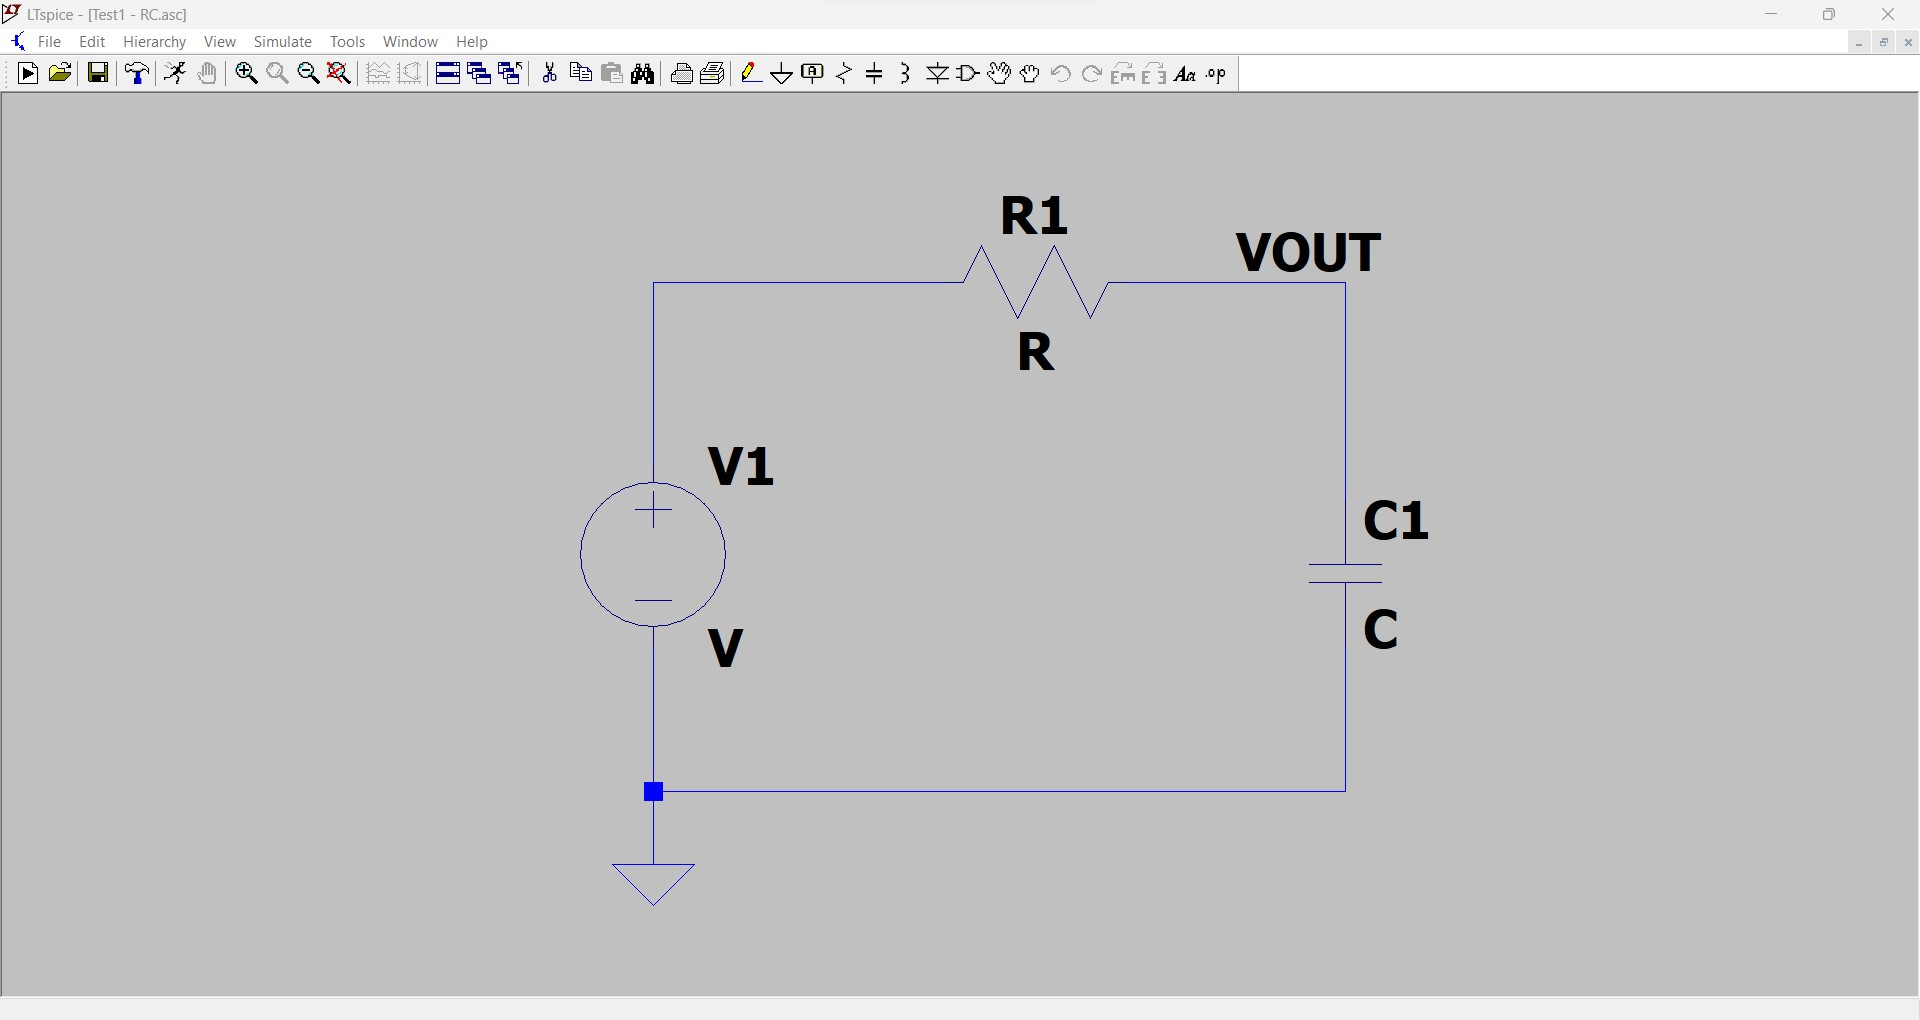
\includegraphics[width=0.75\textwidth]{./ImageFiles/LTSpice.jpg}
	\caption{Schermata principale di LTSpice.}
	\label{fig:ltspice}
\end{figure}
\newpage
\noindent
Il motore di simulazione è basato sul programma SPICE (\textit{Simulation Program with Integrated Circuit Emphasis}) che riceve in input una \texttt{netlist}, ossia una rappresentazione testuale del circuito, e produce in output i risultati di simulazione. LTSpice crea automaticamente la \texttt{netlist} a partire dalla rappresentazione grafica del circuito. Per esempio, il circuito in figura \ref{fig:ltspice} genera la seguente netlist:
\lstinputlisting[language=Octave]{./OtherFiles/netlist.txt}
Inoltre, il programma salva il circuito in un file con estensione .asc che contiene tutte le informazioni per rappresentare in modo grafico il circuito. Di seguito si riporta il file .asc prodotto dal circuito in figura \ref{fig:ltspice}.
\lstinputlisting[language=Octave]{./OtherFiles/asc.txt}
Come si può notare, in questo file non vengono riportate informazioni sulla simulazione da eseguire ma bensì la posizione dei collegamenti, dei componenti, delle label ed eventuali attributi. In particolare, le principali parole chiave che si possono riconoscere sono:
\begin{itemize}
	\item VERSION: rappresenta la versione del sistema utilizzato; per il progetto verrà considerata solamente la versione 4;
	\item SHEET: definisce il numero del foglio di lavoro utilizzato e le relative dimensioni;
	\item WIRE: indica un filo di collegamento; seguono le coordinate x,y assolute dei relativi capi;
	\item SYMBOL: rappresenta un componente; di seguito si riporta la tipologia, la posizione assoluta in coordinate x,y e l'eventuale rotazione o mirror; è possibile indicare una rotazione di 0°, 90°, 180°, 270° o un'operazione di mirror di 0°, 90°, 180° e 270°;
	\item SYMATTR: permette di indicare eventuali attributi riferiti a un simbolo come il nome, il valore, i parametri dei componenti parassiti o indicare il produttore del componente;
	\item WINDOW: indica la posizione della label associata a un componente (il nome o il valore) nel caso di rotazioni e mirror;
	\item FLAG: definisce la posizione e il contenuto di eventuali label associati a dei collegamenti in un circuito; viene utilizzata anche per indicare la massa (indicando come nome della label 0);
	\item IOPIN: indicano una label di ingresso o uscita nel circuito. 
\end{itemize}
Tutte le coordinate sono espresse attraverso numeri interi e le parole chiave sono interpretate in modo \textit{case insensitive}. Il formato di codifica del file è \texttt{ISO-8859-1} e accetta qualsiasi carattere \texttt{UNICODE} all'interno delle label e dei nomi dei componenti. Le parole chiave e i relativi parametri sono separati da degli spazi bianchi. LTSpice è insensibile al numero di spazi tra i diversi token e di eventuali caratteri di \textit{newline}. Tuttavia, il file .asc in output a LTSpice è formattato mantenendo un unico spazio tra ogni token e andando a capo prima di ogni parola chiave.

\section{ltspice2circuitikz}
L'applicazione finale realizzata in questo progetto si suddivide in due principali componenti:
\begin{itemize}
	\item un'interfaccia grafica, realizzata con il framework Qt;
	\item un'applicazione Java che realizza le operazioni necessarie per la traduzione, distribuita come un .jar eseguibile.
\end{itemize}
In figura \ref{fig:deploy_diagram} è mostrato il deploy diagram dell'intera applicazione.
\begin{figure}[h!]
	\centering
	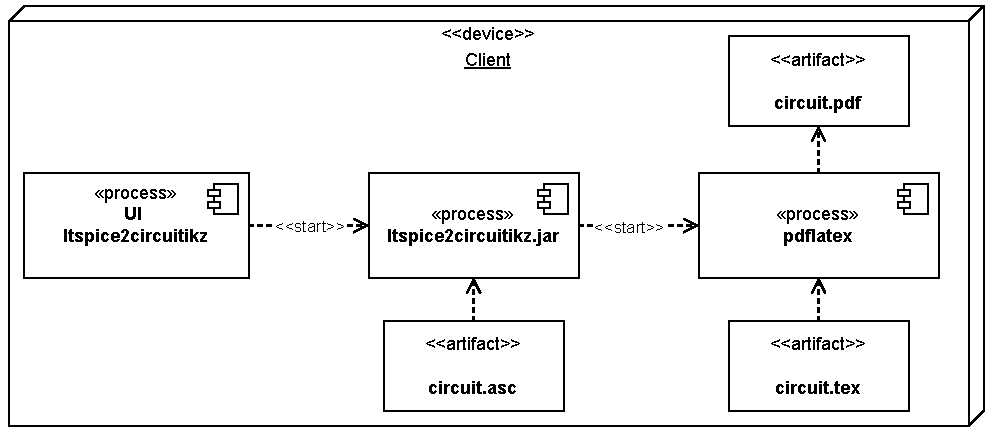
\includegraphics[width=0.5\textwidth]{./ImageFiles/deploy diagram.pdf}
	\caption{Deploy diagram del sistema.}
	\label{fig:deploy_diagram}
\end{figure}

\noindent
L'interfaccia utente (\texttt{UI ltspice2circuitikz}) avvia l'applicativo jar (\texttt{ltspice2circuitikz.jar}), il quale richiede in input il file .asc contente la specifica del circuito realizzata con LTSpice. A sua volta, l'applicazione Java, una volta terminata la traduzione, avvia il processo \texttt{pdflatex} che richiede in input il file .tex ottenuto dalla traduzione e restituisce il pdf con la rappresentazione del circuito.

\noindent
In figura \ref{fig:class_diagram} viene mostrato il diagramma delle classi e dei package dell'applicazione Java.
\begin{figure}[h!]
	\centering
	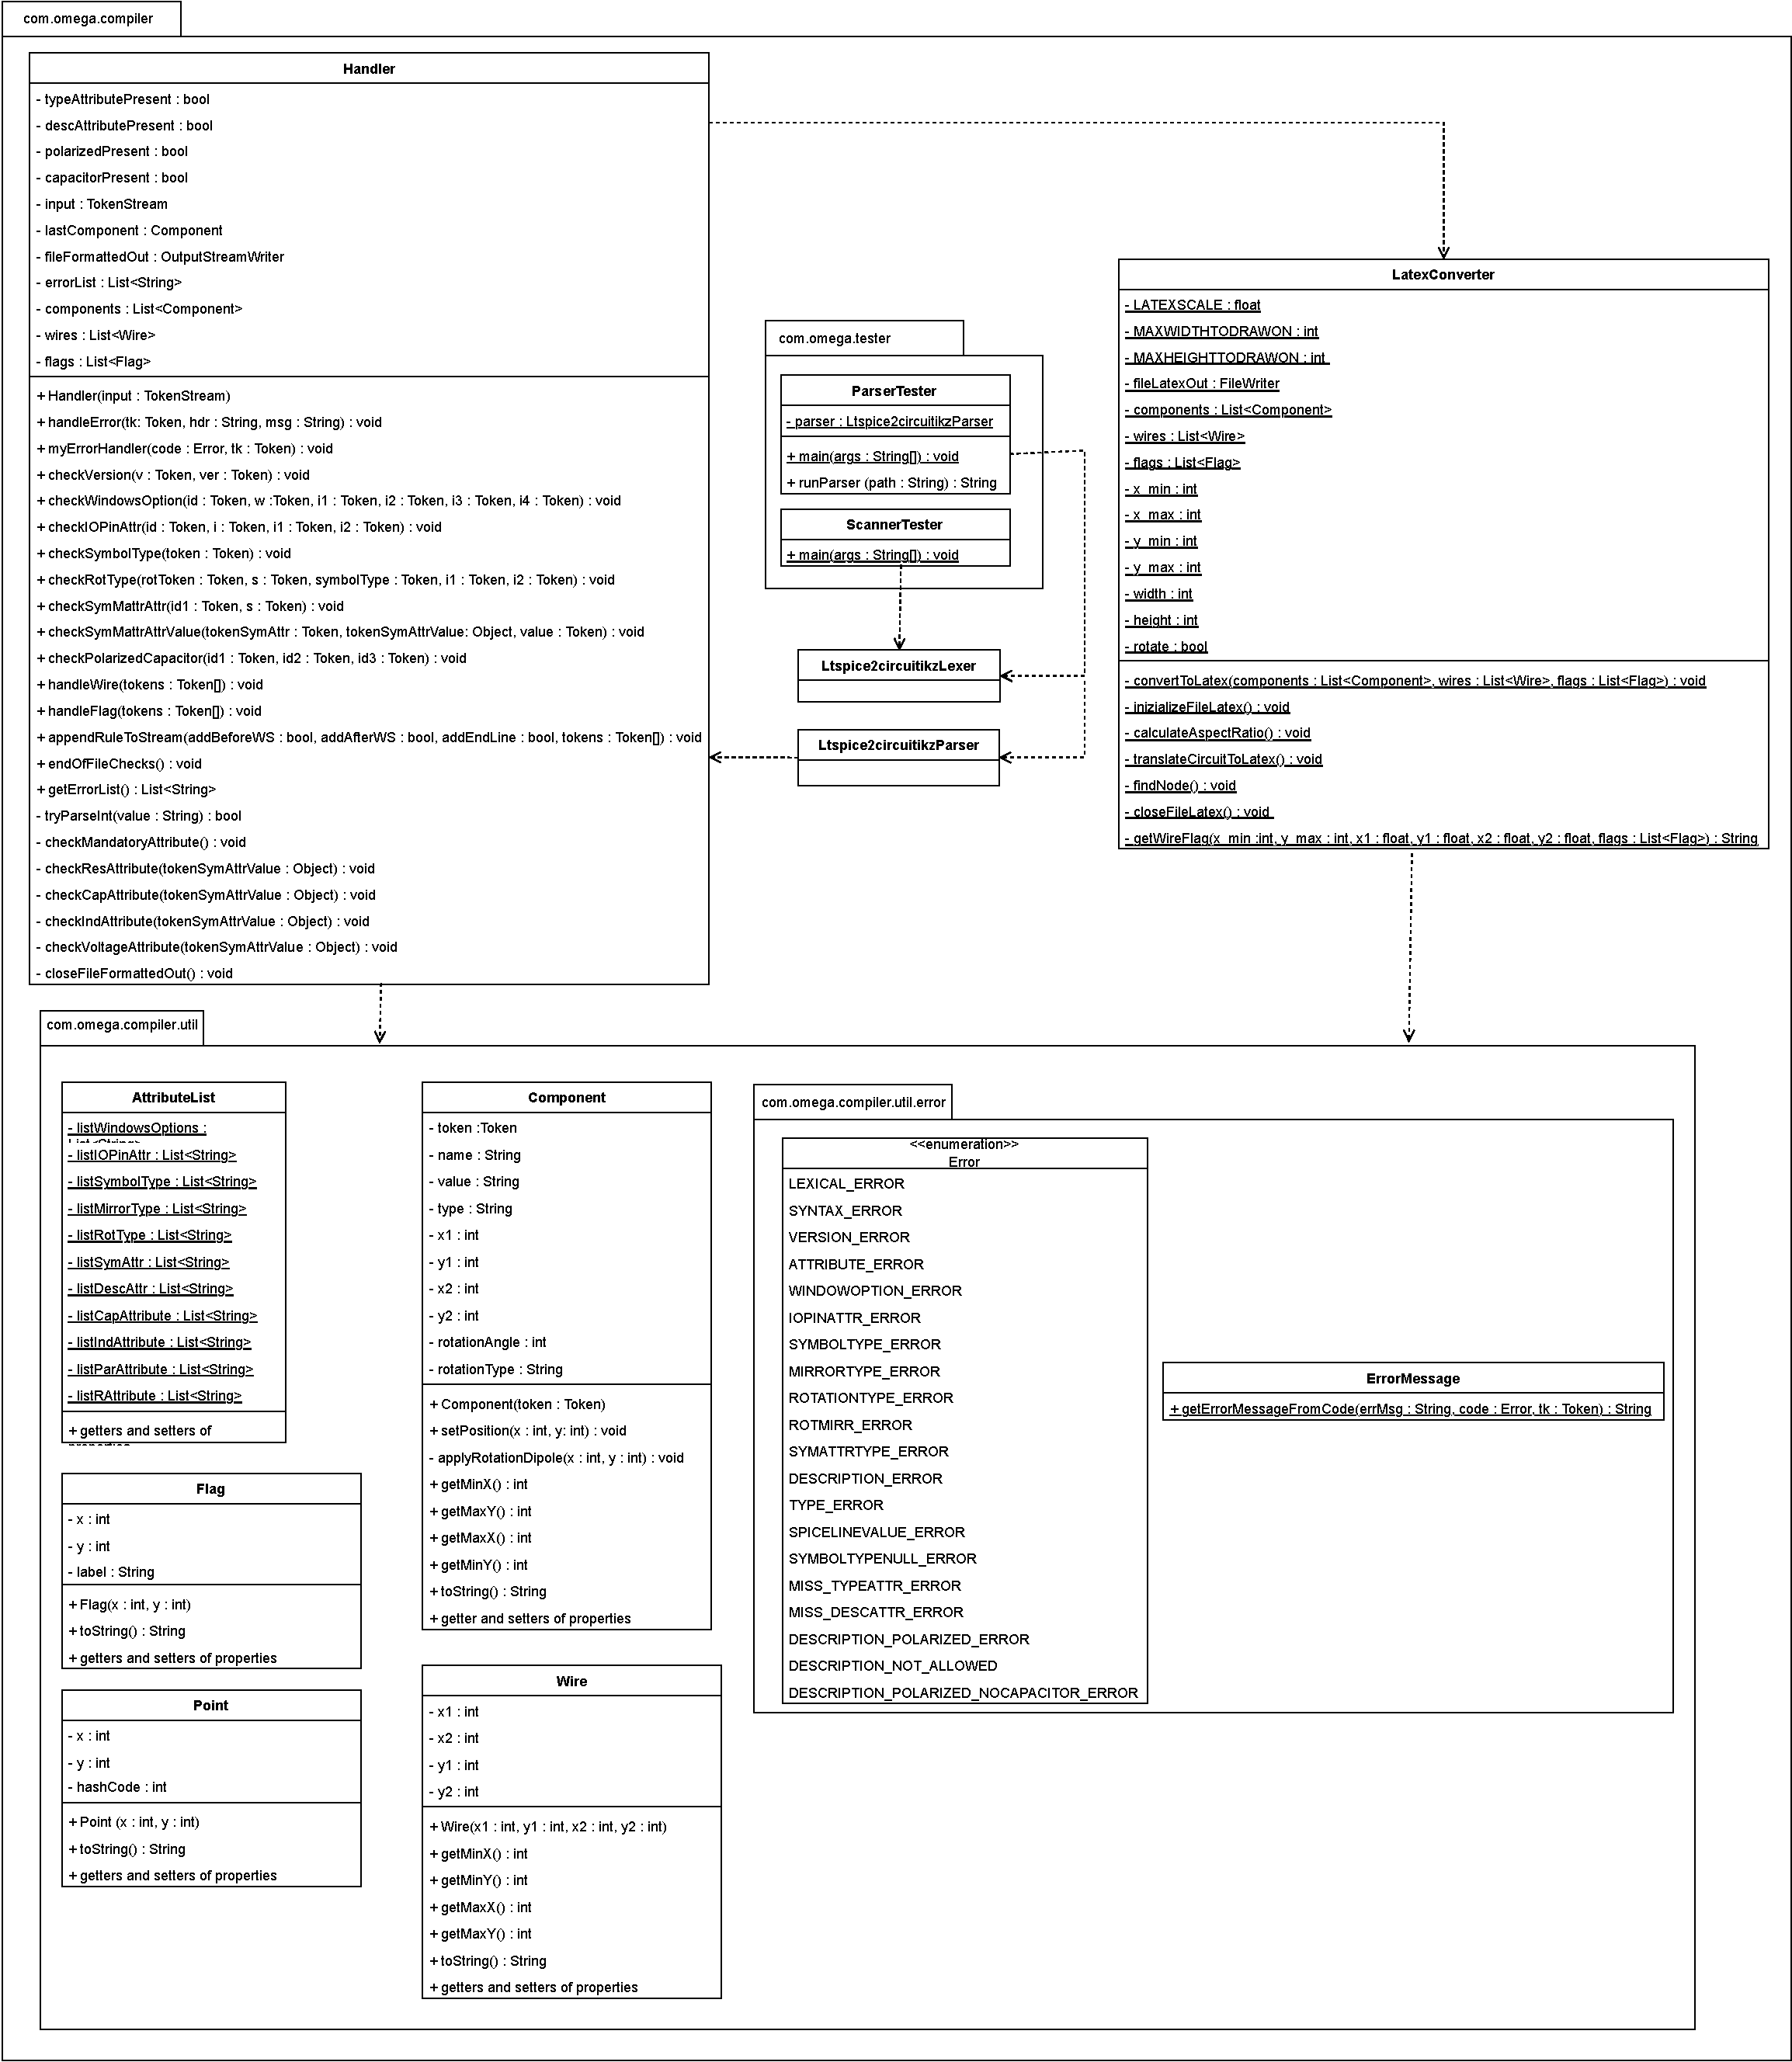
\includegraphics[width=\textwidth]{./ImageFiles/class and package diagram.pdf}
	\caption{Class and Package Diagram dell'applicazione.}
	\label{fig:class_diagram}
\end{figure}
Il metodo \texttt{main} richiamato all'avvio dell'applicazione è contenuto nella classe \texttt{ParserTester}, la quale contiene i riferimenti al lexer e al parser generato da \texttt{ANTLRWorks}. Inoltre, il parser contiene il riferimento alla classe \texttt{Handler} che fornisce i metodi per eseguire le azioni semantiche. Il package \texttt{com.omega.compiler.util} contiene alcune classi utilizzate dalle azioni semantiche per descrivere un componente (classe \texttt{Component}), un collegamento (\texttt{classe Wire}), una label (classe \texttt{Flag}), un nodo (classe \texttt{Point}) e gli errori. La classe \texttt{LatexConverter} si occupa invece di effettuare le operazioni di traduzione e di creazione del file latex. I metodi contenuti vengono richiamati dalla classe \texttt{Handler}.

\clearpage
\subsubsection{Lexer e Parser}
L'applicazione realizzata si basa su un lexer e un parser LL(1) generato nel linguaggio Java grazie al tool \texttt{AntlrWorks}. Essi permettono di leggere ed interpretare un file .asc e di effettuare la traduzione in un file .tex tramite delle azioni semantiche. Per definire la grammatica utile al parsing del file .asc è stato eseguito un processo di \textit{reverse engeneering}, analizzando il file generato da LTSpice con dei circuiti di esempio. Di seguito si riportano i token identificati e le regole sintattiche ricavate dall'analisi dei file .asc.
\lstinputlisting[]{./OtherFiles/grammatica non decorata.txt}
In particolare, si è notato che il programma non generava errore all'apertura del file se:
\begin{itemize}
	\item le parole chiave erano scritte in caratteri minuscoli o in una qualsiasi combinazione di caratteri minuscoli e maiuscoli;
	\item venivano aggiunti degli spazi bianchi o dei caratteri di terminazione di riga tra le parole;
\end{itemize}
Per mantenere coerente la grammatica con questo comportamento, è stato considerato come separatore tra i diversi token il carattere di spazio bianco, di terminazione di riga e di tab. Inoltre, le parole chiave sono state rese invarianti rispetto al carattere delle lettere (lower o upper case). La grammatica completa si compone di nove parole chiavi: VERSION, SHEET, WIRE, SYMBOL, SYMATTR, simbolo di assegnamento (=), WINDOW e IOPIN. Ulteriori controlli sulle possibili strutture ammesse sono state inserite nella semantica, discussa successivamente. Inoltre, LTSpice accetta l'inserimento di qualunque carattere \texttt{UNICODE} nelle label dei componenti. Per questo motivo sono stati aggiunti i token per il riconoscimento dei caratteri speciali, dell'alfabeto greco e dell'alfabeto cirillico.

\subsection{Semantica}
Per gestire le azioni semantiche è stata predisposta la classe \texttt{Handler} che racchiude la definizione dei metodi utilizzati per i controlli semantici e le operazioni di traduzione. Di seguito si riporta la grammatica decorata con le operazioni semantiche.
\lstinputlisting[]{./OtherFiles/grammatica decorata.txt}

\noindent
Nel costruttore della classe \texttt{Handler} vengono dapprima inizializzate alcune strutture dati che verranno utilizzate per gestire la traduzione. In particolare, vengono create le liste \texttt{components}, \texttt{wires} e \texttt{flags} che servono a memorizzare i componenti letti in modo incrementale durante l'analisi del file in input; viene inizializzata anche una lista che conterrà gli errori lessicali, sintattici e semantici. Inoltre, viene creata una cartella con il nome \texttt{circuit\_output} e un file denominato \texttt{formatted\_circuit.asc} che conterrà la descrizione del circuito in formato LTSpice formattato correttamente. Infatti, come già descritto in precedenza, l'inserimento di spazi bianchi e caratteri di terminazione di linea non precludono la possibilità di interpretare correttamente il file. Per questo motivo, ogni qualvolta viene letto un token o un'insieme di token essi sono accodati al file \texttt{formatted\_circuit.asc} grazie alla funzione \texttt{appendRuleToStream} dichiarata nell'handler. Questa funzione ha come argomenti l'insieme dei token da scrivere sul file e alcuni parametri booleani per descrivere come devono essere formattati nel file (aggiungere uno spazio prima o dopo ogni token e al termine della riga scritta il carattere di \textbackslash n). 

\noindent
Un altro campo importante nella classe \texttt{Handler} è \texttt{lastComponent}. Esso è di tipo \texttt{Component}, una classe contenuta nel package \texttt{com.omega.compiler.util} che contiene tutte le informazioni relative a un componente. Questa variabile è utilizzata per mantenere memoria dell'ultimo componente letto: in questo modo, è possibile poi effettuare dei controlli sulle regole che vengono lette successivamente e che si riferiscono a quel componete. Essa viene inizializzata nel metodo \texttt{checkSymbolType} chiamato quando si incontra la parola chiave \texttt{SYMBOL} nella regola sintattica \texttt{symbolRule}.

\noindent
Al termine della lettura di tutto il contenuto del file .asc in input, se non ci sono stati errori, viene chiamato il metodo statico \texttt{convertToLatex} della classe \texttt{LatexConverter} che inizia il processo di traduzione. Inoltre, si procede alla chiusura del file \texttt{formatted\_circuit.asc}.

\subsection{Traduzione}
La classe \texttt{LatexConverter} contiene i metodi necessari alla traduzione del circuito per la rappresentazione in Latex. Il metodo \texttt{convertToLatex}, chiamato dall'handler, riceve in ingresso la lista dei componenti, dei collegamenti e delle etichette ricavate dal file in ingresso. Successivamente, viene chiamato il metodo \texttt{calculateAspectRatio} che consente di calcolare i valori massimi e minimi delle coordinate x e y di tutti gli elementi del circuito e viene calcolata l'altezza e la larghezza del circuito nel sistema di riferimento di LTSpice. Se l'altezza è minore della larghezza allora il circuito verrà rappresentato su un foglio in modalità \textit{landscape}. Nella figura \ref{fig:sdr} sono mostrati i sistemi di riferimento utilizzati in LTSpice e in Latex. Non è conosciuta la posizione assoluta del sistema di riferimento in LTSpice rispetto alla finestra visualizzata.
\begin{figure}[h!]
	\centering
	a)
	\begin{minipage}{.460\textwidth}
		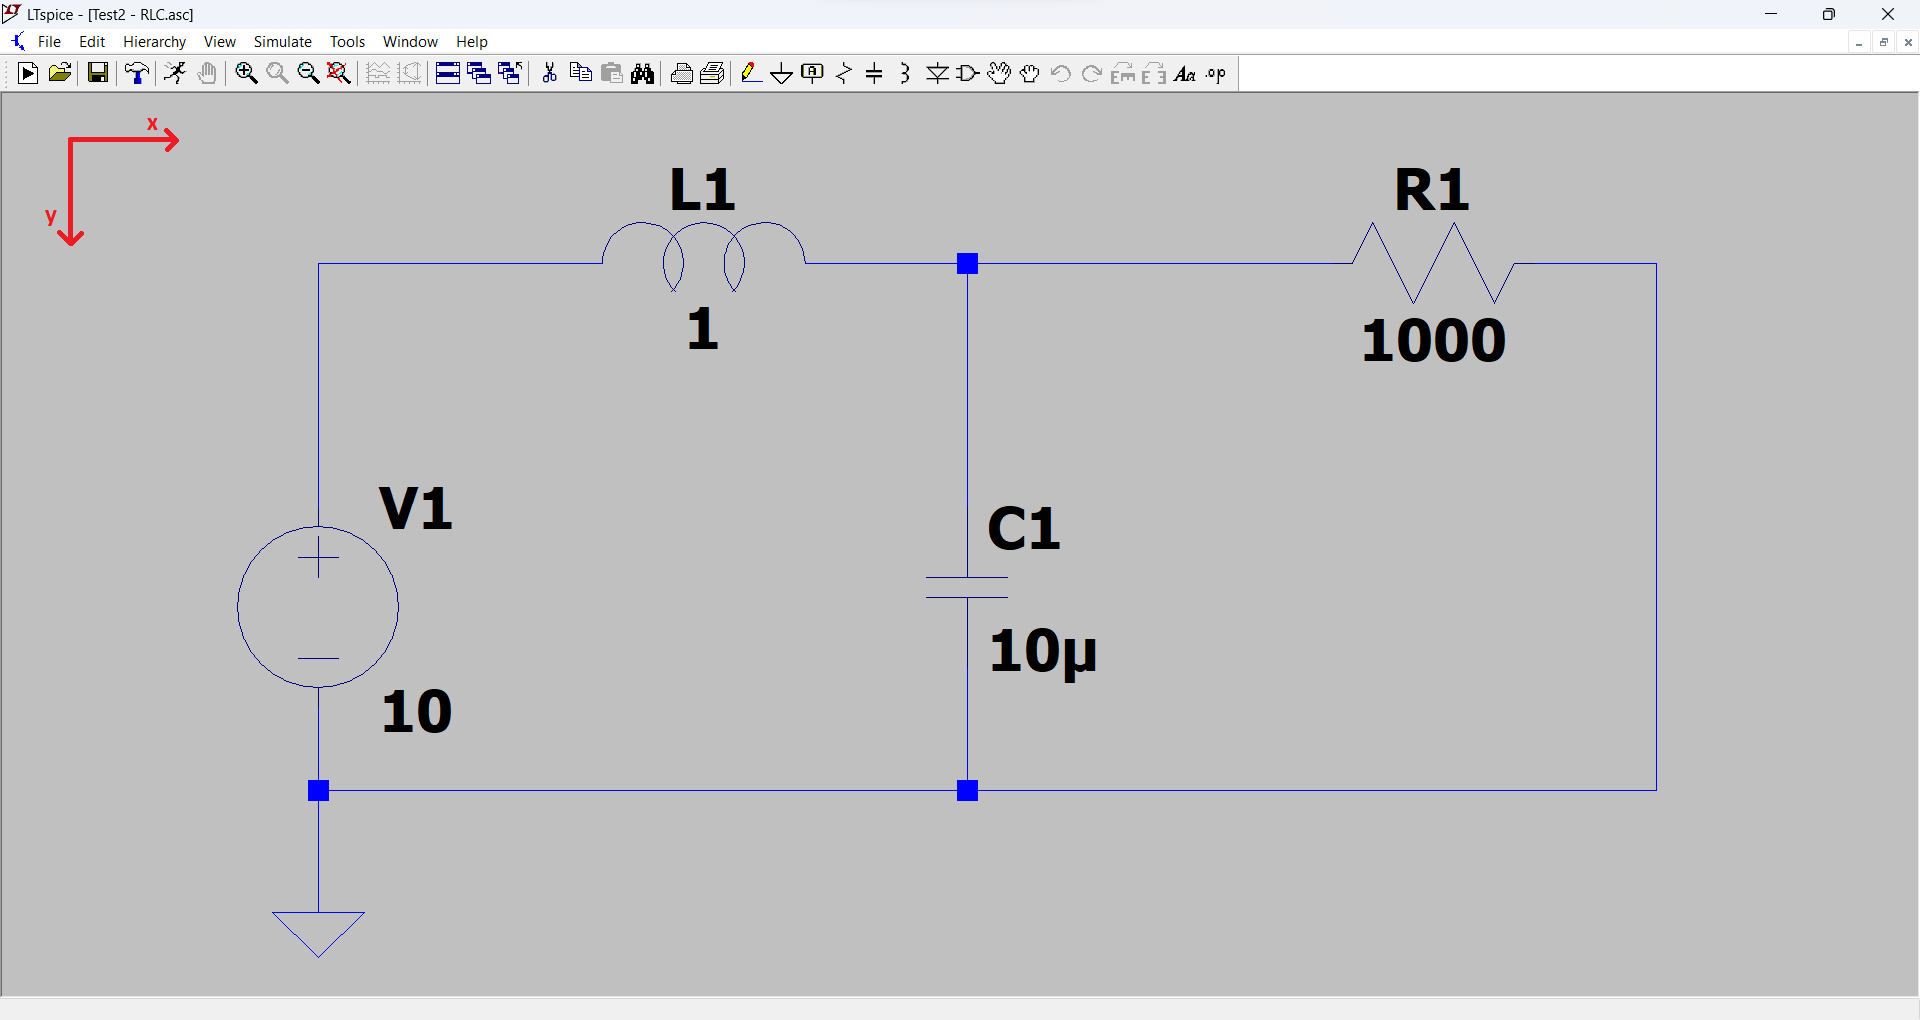
\includegraphics[width=\linewidth]{./ImageFiles/sdr-lt.png}
	\end{minipage}
	b)
	\begin{minipage}{.460\textwidth}
		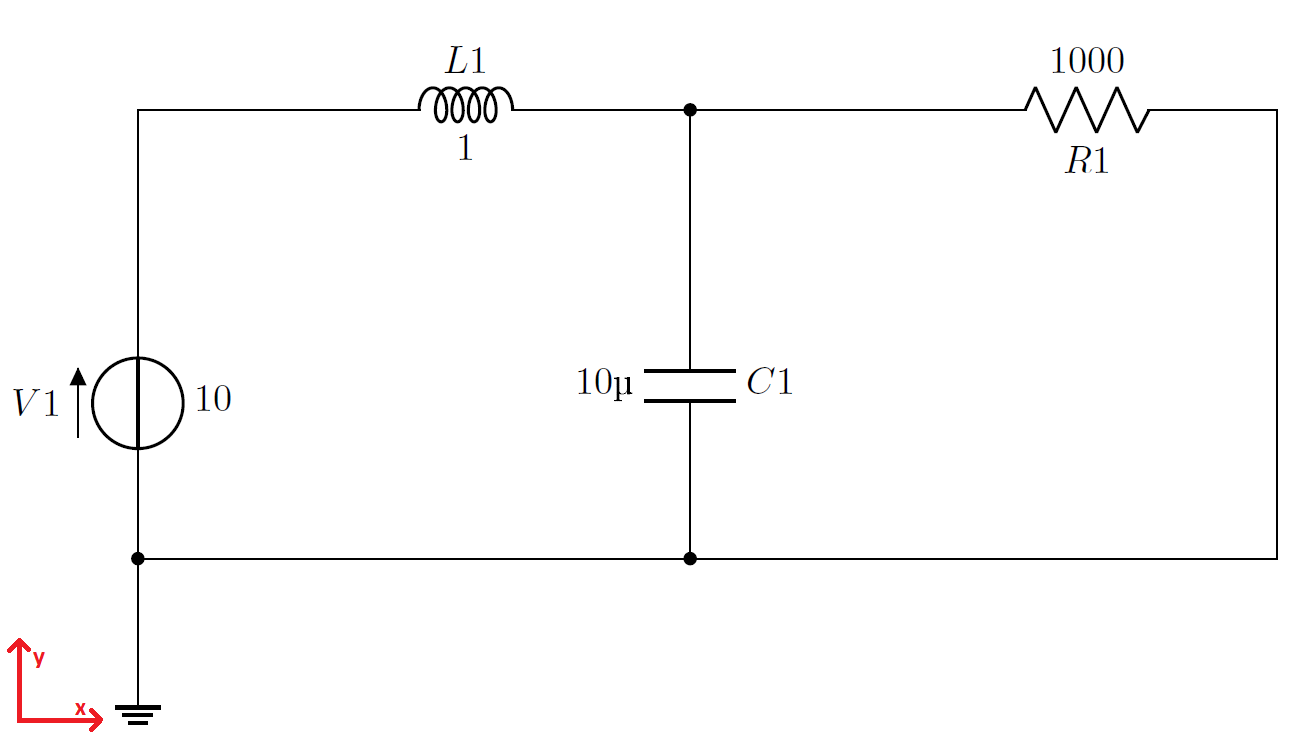
\includegraphics[width=\linewidth]{./ImageFiles/sdr-latex.png}
	\end{minipage}
	\caption{Sistemi di riferimento delle coordinate x e y in LTSpice e in Latex.}
	\label{fig:sdr}
\end{figure}

\noindent
Viene quindi creata la cartella \texttt{latex\_output} e il file \texttt{translated\_circuit.tex} che conterrà la traduzione in Latex del circuito. Dapprima, viene scritto nel file latex il preambolo che contiene la descrizione del tipo di documento, la dimensione del foglio e l'import del pacchetto \texttt{CircuiTikz}. Queste informazioni verranno utilizzate dal compilatore \texttt{MikTex} durante la generazione del file pdf.

\noindent
Il passo successivo consiste nella vera e propria traduzione del circuito in Latex effettuata dalla funzione \texttt{translateCircuitToLatex}. Inizialmente, vengono calcolate altezza e larghezza del circuito e nel caso in cui lo schematico sia più largo che alto viene impostata la variabile \texttt{rotate} che ruota il circuito in modo da occupare meglio lo spazio. Poi, viene calcolato il fattore di scala (memorizzato nella variabile \texttt{LATEXSCALE}) tra le coordinate espresse nel sistema di riferimento di LTSpice e quello di Latex, in modo tale che il circuito tradotto sia contenuto interamente in un unico foglio. Successivamente, vengono tradotti tutti i componenti, i collegamenti e le label inserite nelle liste \texttt{components}, \texttt{wires} e \texttt{flags}; questa operazione richiede di recuperare le coordinate x e y degli estremi di collegamento di ogni componente ed effettuare una rototraslazione per riportare le coordinate dal sistema di riferimento di LTSpice nel sistema di riferimento di Latex: alla coordinata x viene sottratta la x minima calcolata nella funzione \texttt{calculateAspectRatio} mentre alla y viene sottratta la coordinata y massima, anch'essa calcolata precedentemente. Le coordinate y vengono poi invertite. Infine, tutte le coordinate vengono scalate con il fattore di scala \texttt{LATEXSCALE} calcolato precedentemente. Il comando Latex utilizzato per disegnare un componente secondo la libreria \texttt{CircuiTikz} è \texttt{draw} ed è così definito:
\begin{itemize}
	\item \textbackslash draw (x1,y1) to[$\langle$type$\rangle$=$\langle$name$\rangle$, a=$\langle$value$\rangle$] (x2,y2), per disegnare un componente; il $\langle$type$\rangle$ può essere R, C, eC, L, Do o vsource per indicare una resistenza, un capacitore, un capacitore polarizzato, una induttanza, un diodo e un generatore di tensione; $\langle$name$\rangle$ e $\langle$value$\rangle$ corrispondono al nome e al valore del componente; le coordinate degli estremi vengono calcolate a partire dalle coordinate x,y del componente indicate nel file .asc che fanno riferimento al centro del componente; a queste coordinate vengono applicati degli offset (ricavati sperimentalmente) per calcolare la posizione dei capi di collegamento in funzione anche della rotazione o operazione di mirror applicata; queste operazioni sono inserite nella funzione \texttt{applyRotationDipole} nella classe \texttt{Component};
	\item \textbackslash draw (x1,y1) to[short, l=$\langle$label$\rangle$] (x2,y2), traccia un filo di collegamento dal punto (x1,y1) al punto (x2,y2) e associa eventualmente una label $\langle$label$\rangle$ al collegamento; questa label viene ricercata nella lista \texttt{flags}, cercando una flag che abbia le stesse coordinate di uno dei capi del collegamento;
	\item \textbackslash draw (x,y) to (x,y) node[ground]{}, inserisce un nodo di massa nel punto (x,y); i nodi di massa in LTSpice sono rappresentati da dei flag con valore 0;
	\item \textbackslash draw (x,y) to[short, -*] (x,y), permette di rimarcare un nodo come punto di collegamento tra tre fili; essi vengono ricavati cercando l'intersezione di almeno tre collegamenti grazie alla funzione \texttt{findNode};
\end{itemize}
Dopo aver terminato la traduzione, la funzione \texttt{closeFileLatex} esegue le operazioni di chiusura del file latex, dopo aver inserito l'epilogo latex. Successivamente, crea un nuovo processo \texttt{pdflatex} al quale passa il nome del file (\texttt{translated\_circuit.tex}) da cui generare il pdf. Se l'operazione va a buon fine, viene prodotto nella cartella \texttt{latex\_output} il pdf con la rappresentazione del circuito.

\noindent
Gli eventuali errori lessicali, sintattici e semantici vengono raccolti nella lista \texttt{errorList} dell'handler. Il metodo \texttt{main}, contenuto nella classe \texttt{ParserTester}, chiama il metodo \texttt{parseCircuit} dichiarato nella classe \texttt{Ltspice2circuitikzParser} che avvia l'analisi sintattica e le operazioni di traduzione. Al termine, viene verificato se la lista \texttt{errorList} è vuota. In tal caso l'applicazione termina. Altrimenti, vengono eliminate le cartelle \texttt{circuit\_output} e \texttt{latex\_output} e viene creata la cartella \texttt{logs} che conterrà un file sul quale vengono scritti gli errori rilevati.

\section{Gestione degli errori}
L'applicazione gestisce sia errori sintattici che errori semantici. Di seguito sono riportati i codici degli errori semantici gestiti dall'applicazione con il loro significato:
\begin{itemize}
	\item \texttt{VERSION\_ERROR}: l'applicazione non è in grado di gestire il numero di versione indicato. Al momento, l'applicazione è in grado di gestire solo la versione 4;
	\item \texttt{ATTRIBUTE\_ERROR}: l'attributo inserito non appartiene all'elenco degli attributi permessi;
	\item \texttt{WINDOWOPTION\_ERROR}: l'opzione riguardante la regola \texttt{WINDOW} non è corretta. Sono ammesse le seguenti opzioni: \texttt{Invisibile}, \texttt{Center}, \texttt{Left}, \texttt{Right}, \texttt{Top}, \texttt{Bottom}, \texttt{VCenter}, \texttt{VLeft}, \texttt{VRight}, \texttt{VTop} e \texttt{VBottom};
	\item \texttt{IOPINATTR\_ERROR}: l'attributo associato alla regola \texttt{IOPIN} non è corretto. Sono ammessi i seguenti attributi: \texttt{In}, \texttt{Out}, \texttt{BiDir};
	\item \texttt{SYMBOLTYPE\_ERROR}: il simbolo inserito non è stato riconosciuto. I simboli che al momento vengono riconosciuti dall'applicazione sono \todo{qui bisogna distinguere in simboli non riconosciuti e simboli non ancora implementati}
	\item \texttt{ROTATIONTYPE\_ERROR}: la rotazione definita per il componente non è valida. Le rotazioni accettate sono \texttt{R0}, \texttt{R90}, \texttt{R180} e \texttt{R270};
	\item \texttt{MIRRORTYPE\_ERROR}: l'attributo di mirror definito per il componente non è valido. Gli attributi possibili sono \texttt{M0}, \texttt{M90}, \texttt{M180} e \texttt{M270};
	\item \texttt{ROTMIRR\_ERROR}: l'attributo inserito non indica ne rotazione ne mirror;
	\item \texttt{SYMATTRTYPE\_ERROR}: la parola che segue il token \texttt{SYMATTR} non è corretta. Le parole ammesse sono \texttt{InstName}, \texttt{Description}, \texttt{Type}, \texttt{Value}, \texttt{SpiceLine};
	\item \texttt{DESCRIPTION\_ERROR}: la parola che segue l'attributo \texttt{Description} deve essere coerente con il simbolo in questione;\todo{Spiegare che se c'è diode allora bla bla se c'è coso allora bla bla}
\end{itemize}

\section{Client app}
L'applicazione client è stata sviluppata utilizzando le librerie Qt 6.4.3 e l'ambiente di sviluppo Qt Creator 10.0.1. L'applicazione è stata sviluppata per sistema operativo Windows, ma grazie alle librerie Qt con lo stesso codice è possibile generare eseguibili anche per altri sistemi operativi (Linux, MacOs, Android e IOs). In figura \ref{fig:class_diagram_client} è mostrato il diagramma delle classi dell'applicazione. Il suo funzionamento viene descritto nel Manuale Utente.

\begin{figure}[h!]
	\centering
	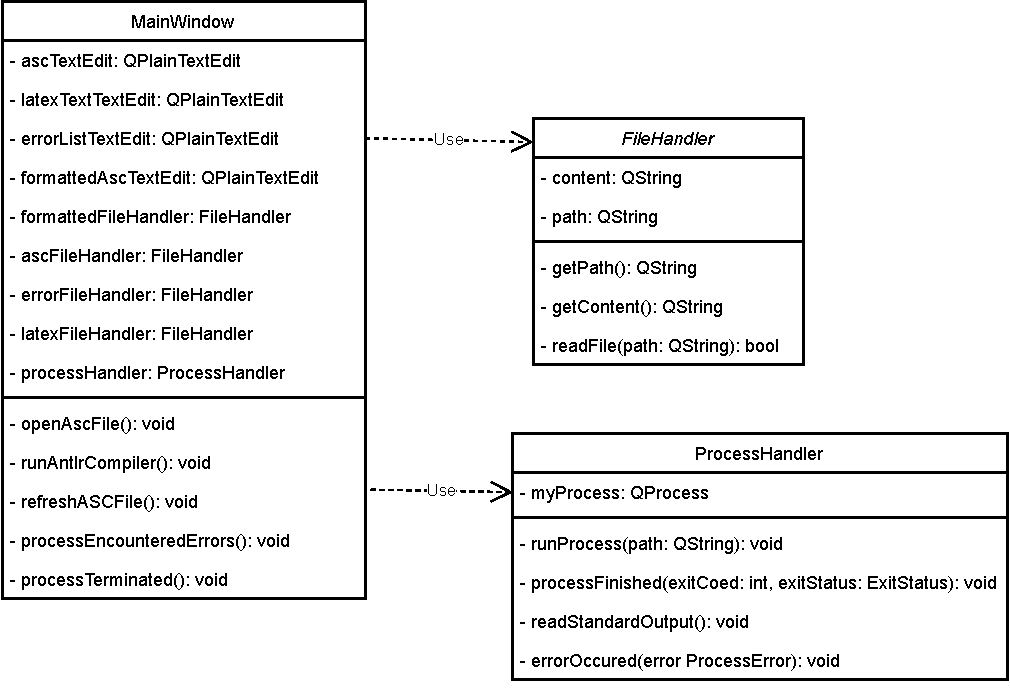
\includegraphics[width=\textwidth]{./ImageFiles/client app diagram}
	\caption{Class Diagram dell'app client.}
	\label{fig:class_diagram_client}
\end{figure}

\clearpage

\section{Esempi e sviluppi futuri}
Di seguito viene riportata una lista contente gli sviluppi futuri:
\begin{itemize}
	\item \textbf{introduzione di nuovi componenti}: al momento, i componenti che possono essere utilizzati sono resistenze, condensatori, condensatori polarizzati, diodi e generatori di tensione. Ci sono altri componenti che possono essere inseriti all'interno dell'applicazione per generare circuiti più complessi.
	\item \textbf{gestione di formati diversi da A4}: al momento, l'applicazione è in grado di disegnare circuiti scalati in modo corretto basandosi sulle dimensioni di un foglio A4. 
	\item \textbf{gestione di fattori di scala molto grandi}: nel caso in cui il circuito sia estremamente grande, l'output generato può contenere dei difetti dovuti al fattore di scala. In tal caso, è consigliabile dividere il circuito su più fogli.
\end{itemize}
Di seguito viene mostrato come utilizzare l'applicazione \textit{ltspice2circuitikz}. 
	\begin{enumerate}
	\item Aprire l'applicazione \textit{ltspice2circuitikz} cliccando due volte l'eseguibile \textit{ltspice2circuitikz.exe}. Si aprirà una schermata come quella mostrata in figura \ref{fig:punto_1}.
	\begin{figure}[h!]
		\centering
		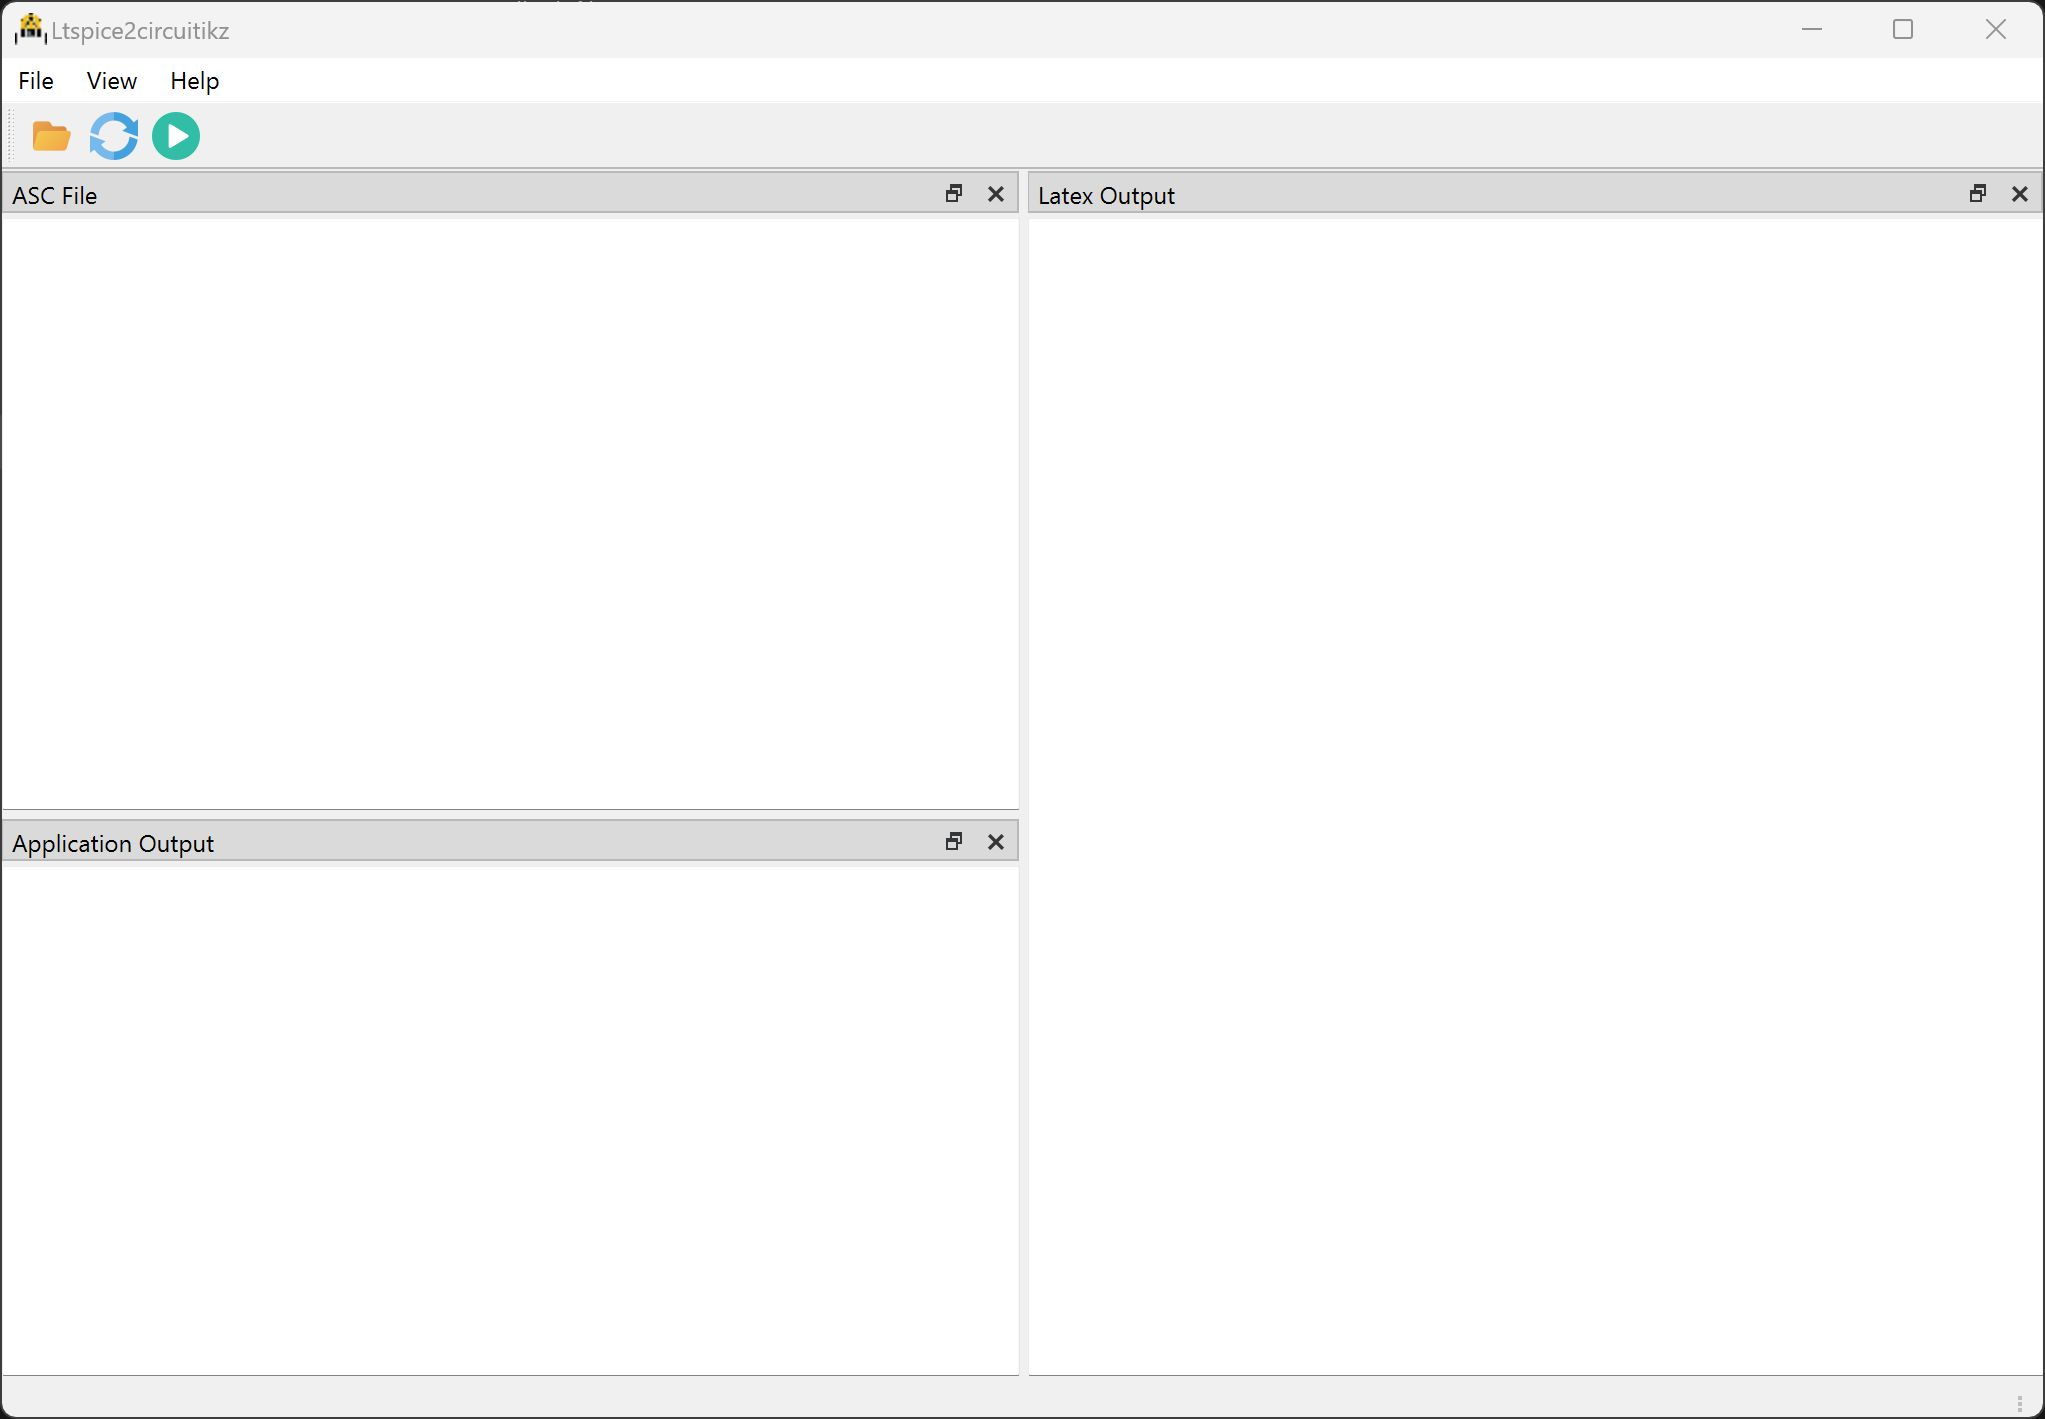
\includegraphics[width=0.7\textwidth]{./ImageFiles/mainview.png}
		\caption{Schermata principale dell'applicazione.}
		\label{fig:punto_1}
	\end{figure}
	\item Cliccare l'icona \textit{"Open File"} e selezionare un file .asc da aprire. Una volta selezionato il file, il suo contenuto verrà mostrato nella finestra in alto a sinistra (figura \ref{fig:punto_2}). Il contenuto del file non può essere modificato dall'applicazione ma deve essere modificato da un tool esterno. Nel caso venga modificato è possibile ricaricare il file premendo l'icona di \textit{"Refresh"}.
	\begin{figure}[h!]
		\centering
		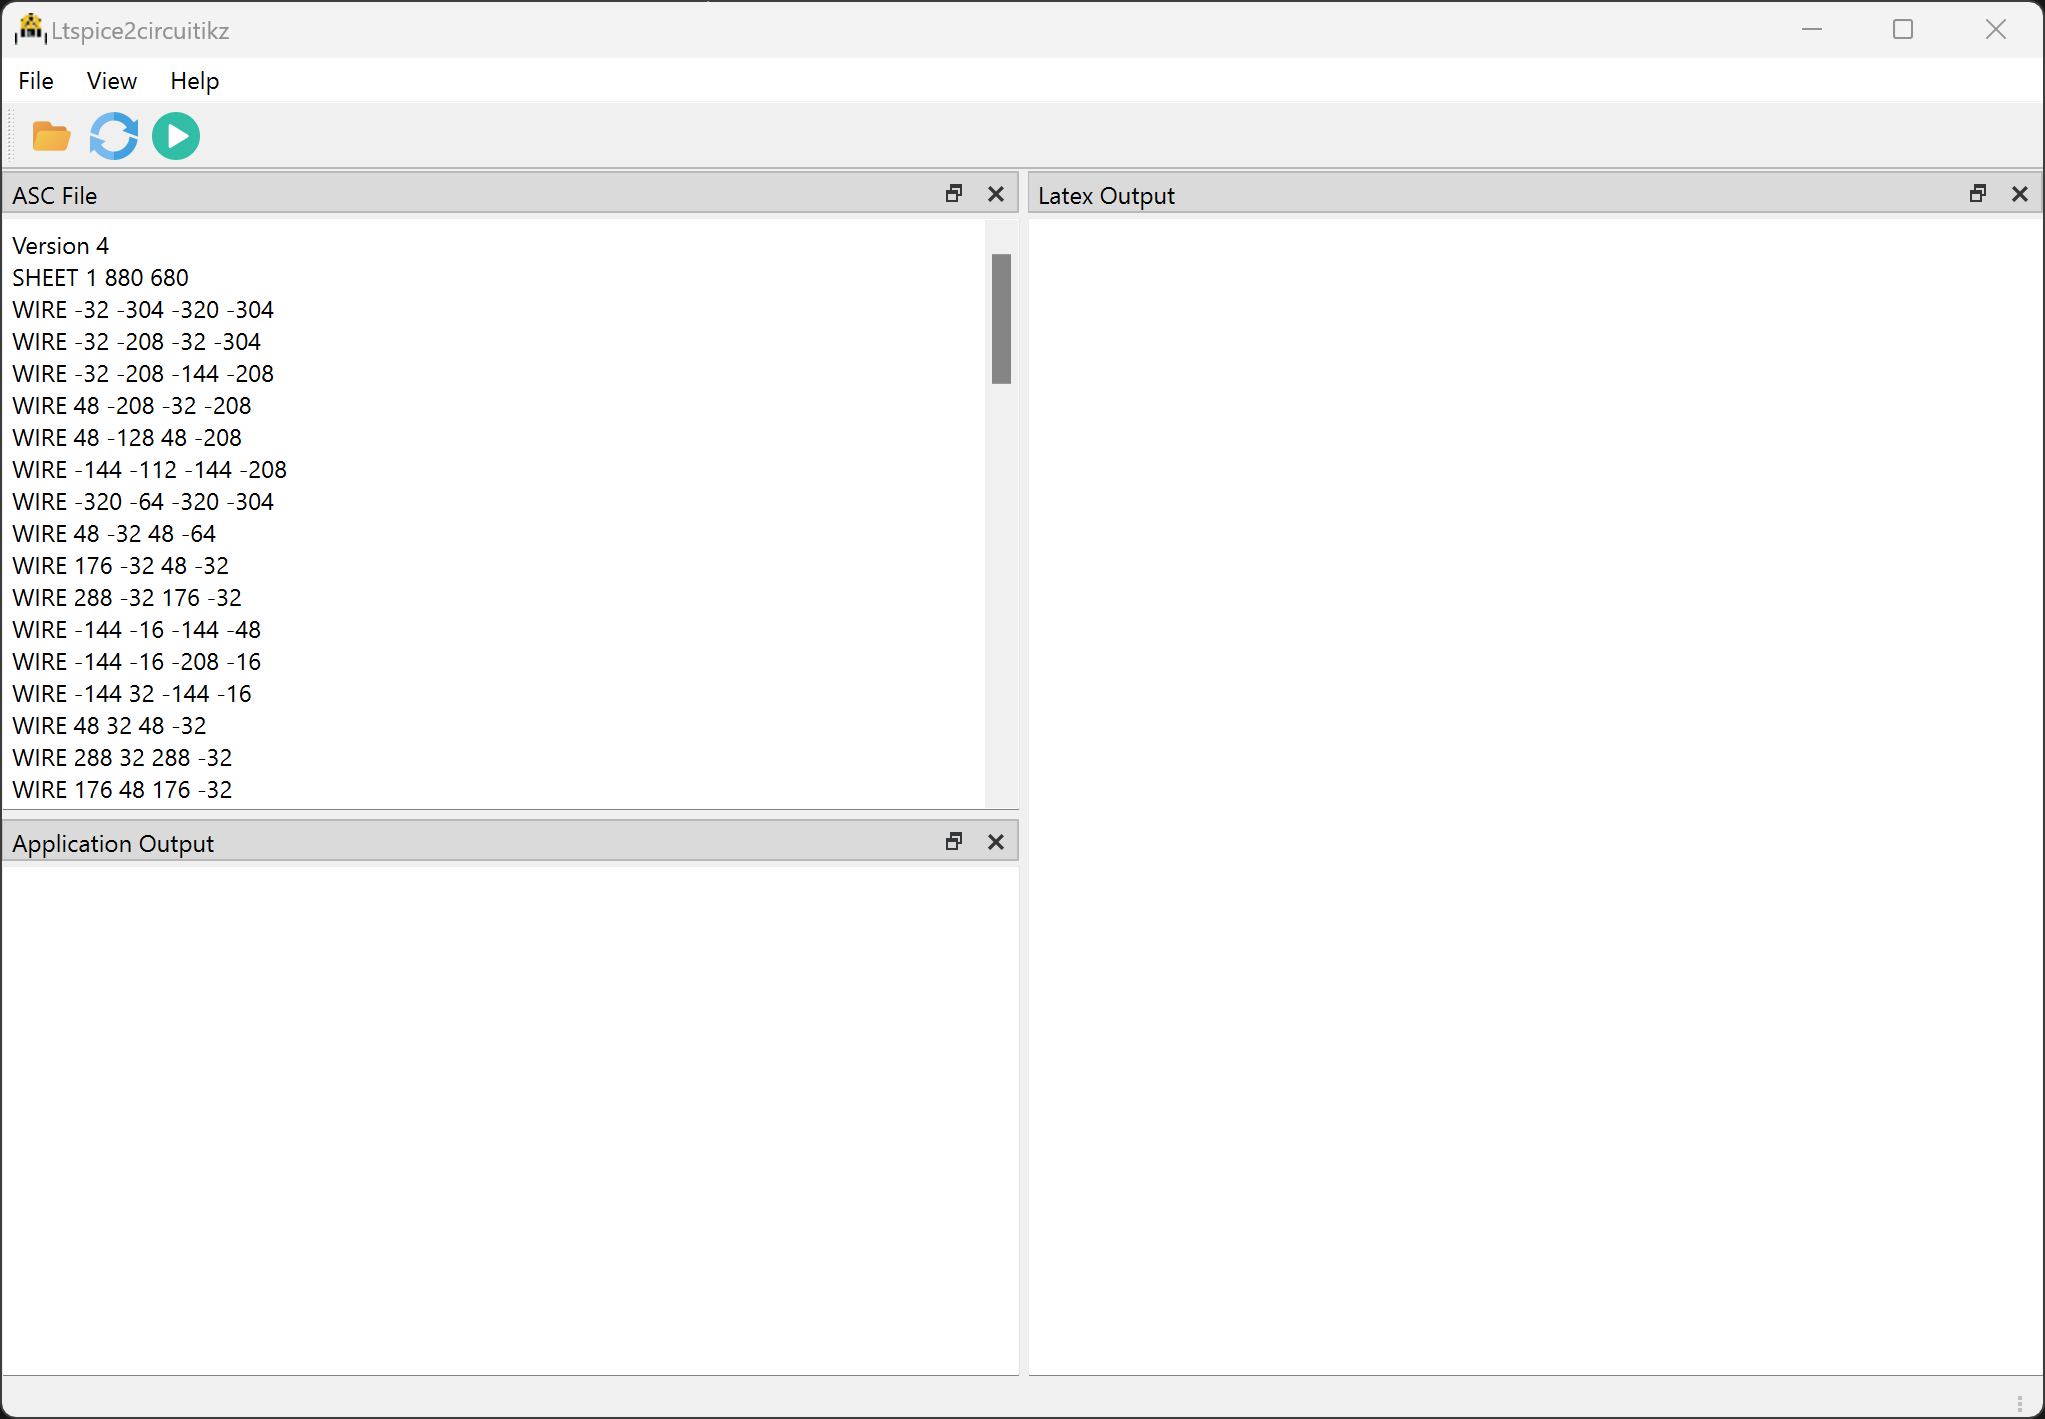
\includegraphics[width=0.7\textwidth]{./ImageFiles/file aperto.png}
		\caption{Schermata che mostra il file aperto.}
		\label{fig:punto_2}
	\end{figure}
	\newpage
	\item Premere il pulsante verde \textit{"Run"} per lanciare il processo di conversione. Se non ci sono errori, viene mostrato un messaggio verde nell'\textit{Application Output} e viene caricato il contenuto del file latex nella colonna di destra (figura \ref{fig:punto_3}). Inoltre, viene aperto il file pdf contenente il circuito generato. Se si vuole mostrare anche il file formattato in modo corretto, è sufficiente selezionare la voce \textit{"Formatted ASC File"} nel menù \textit{"View"}.
	\begin{figure}[h!]
		\centering
		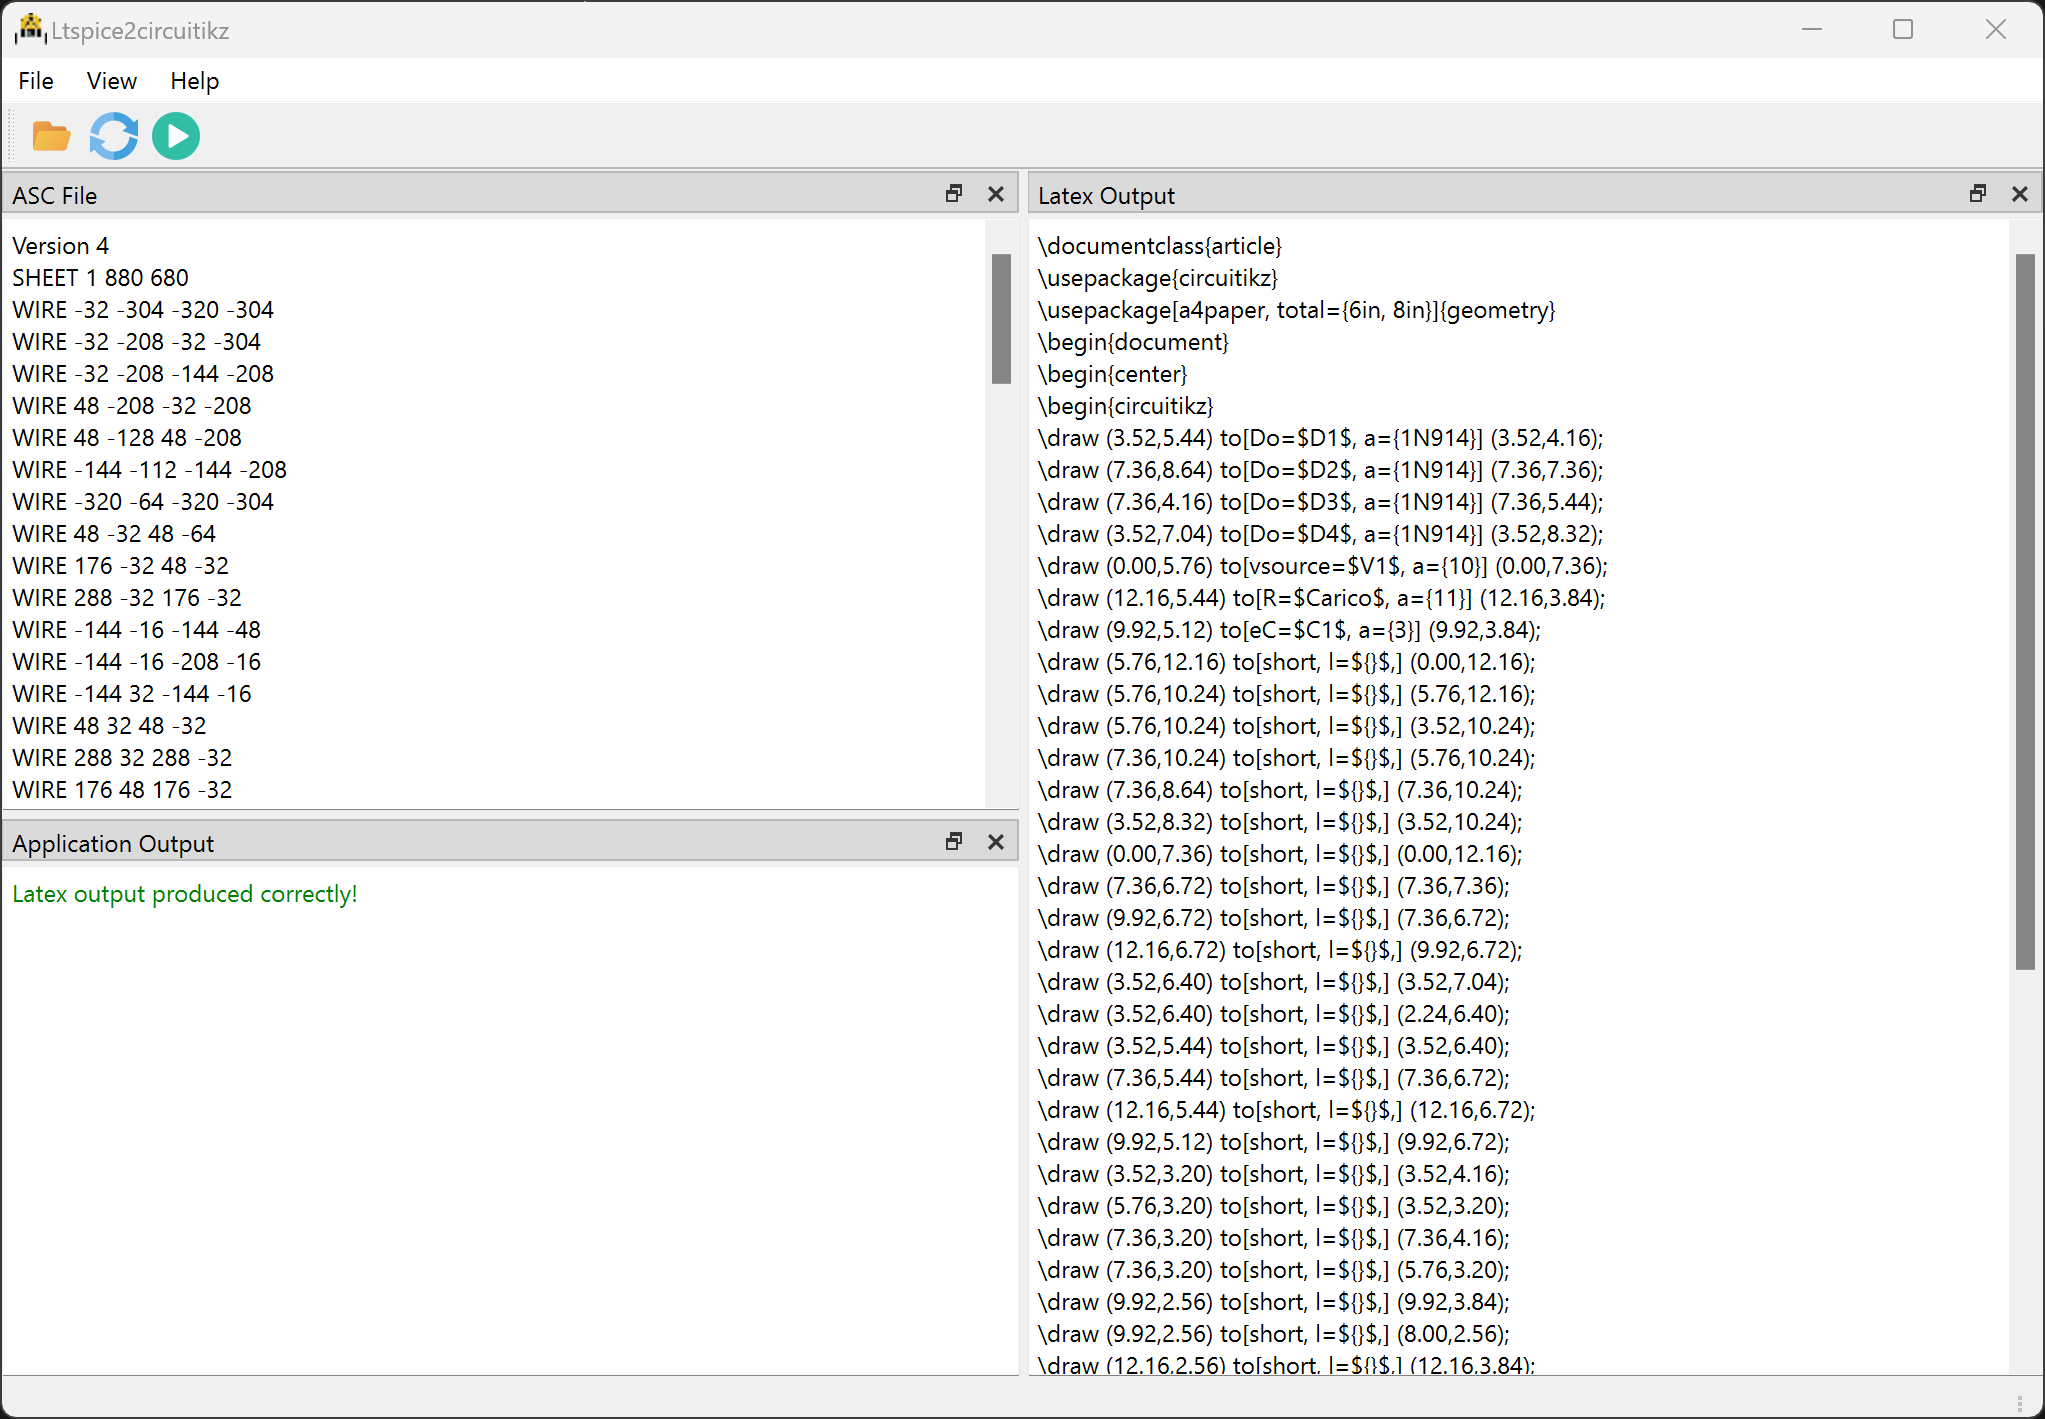
\includegraphics[width=0.7\textwidth]{./ImageFiles/run con successo.png}
		\caption{Processo eseguito con successo.}
		\label{fig:punto_3}
	\end{figure}
	\item Nel caso in cui ci siano errori semantici o sintattici, il processo si interrompe e nell'\textit{Application Output} vengono mostrati gli errori (figura \ref{fig:punto_4}).
	\begin{figure}[h!]
		\centering
		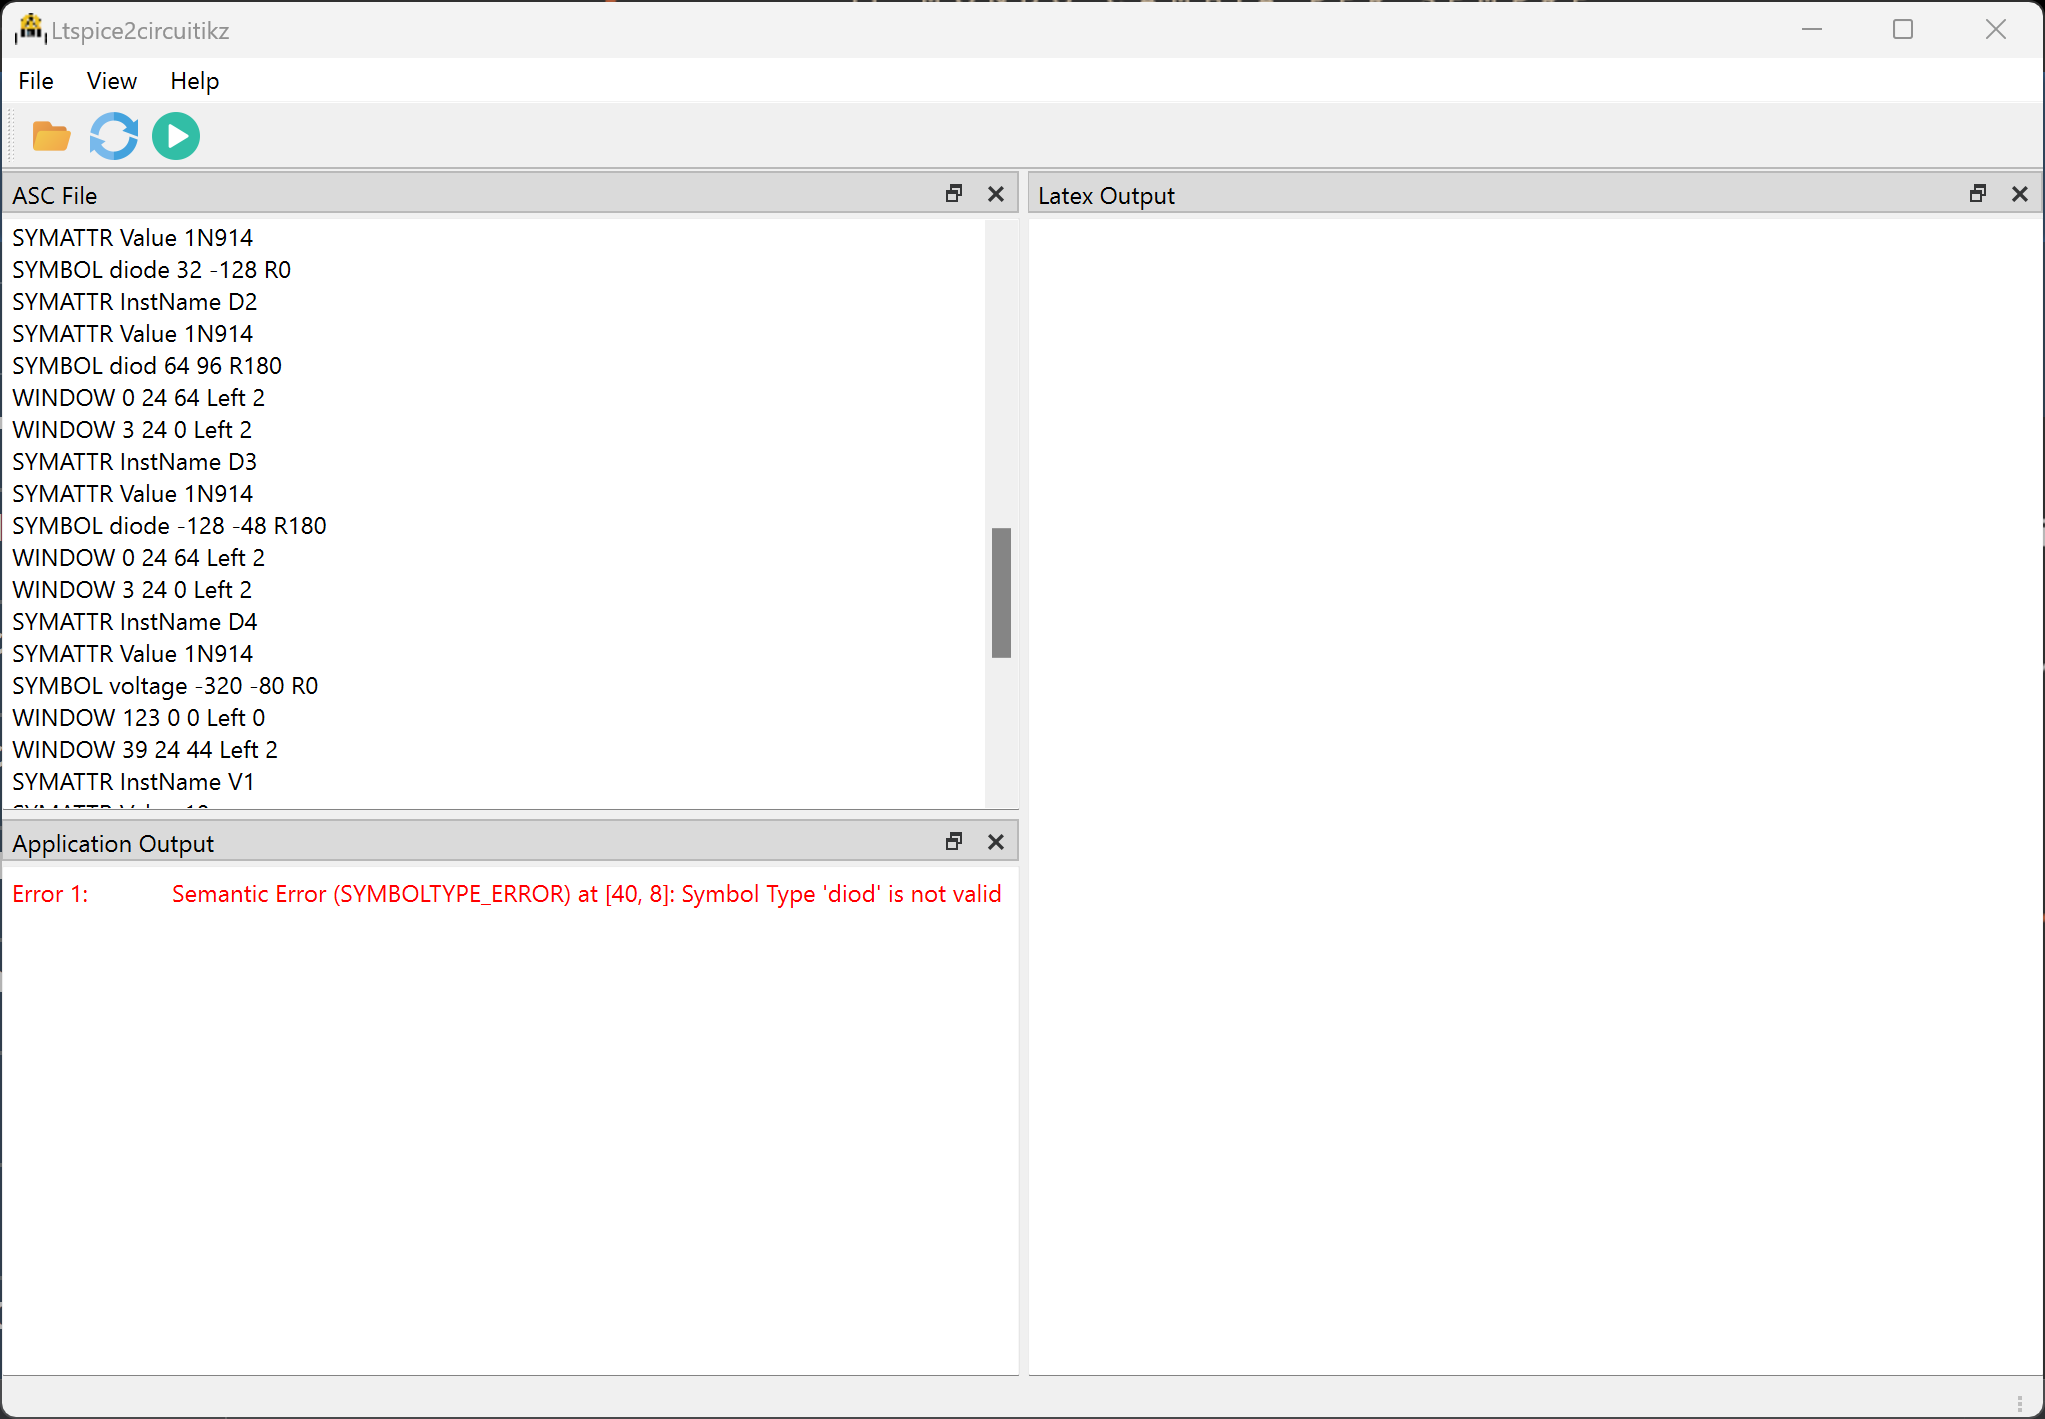
\includegraphics[width=0.7\textwidth]{./ImageFiles/semantic error.png}
		\caption{Errori semantici.}
		\label{fig:punto_4}
	\end{figure}
\end{enumerate}